% --------------------------------------------------------------
% This is all preamble stuff that you don't have to worry about.
% Head down to where it says "Start here"
% --------------------------------------------------------------
 
\documentclass[12pt]{article}
 
\usepackage[margin=1in]{geometry} 
\usepackage{amsmath,amsthm,amssymb}
\usepackage{listings}
\usepackage{enumitem}   
\usepackage{graphicx}
\graphicspath{ {./images/} }

\lstset{
   basicstyle=\fontsize{8}{9}\selectfont\ttfamily
}
 
\newcommand{\N}{\mathbb{N}}
\newcommand{\Z}{\mathbb{Z}}
 
\newenvironment{theorem}[2][Theorem]{\begin{trivlist}
\item[\hskip \labelsep {\bfseries #1}\hskip \labelsep {\bfseries #2.}]}{\end{trivlist}}
\newenvironment{lemma}[2][Lemma]{\begin{trivlist}
\item[\hskip \labelsep {\bfseries #1}\hskip \labelsep {\bfseries #2.}]}{\end{trivlist}}
\newenvironment{exercise}[2][Exercise]{\begin{trivlist}
\item[\hskip \labelsep {\bfseries #1}\hskip \labelsep {\bfseries #2.}]}{\end{trivlist}}
\newenvironment{reflection}[2][Reflection]{\begin{trivlist}
\item[\hskip \labelsep {\bfseries #1}\hskip \labelsep {\bfseries #2.}]}{\end{trivlist}}
\newenvironment{proposition}[2][Proposition]{\begin{trivlist}
\item[\hskip \labelsep {\bfseries #1}\hskip \labelsep {\bfseries #2.}]}{\end{trivlist}}
\newenvironment{corollary}[2][Corollary]{\begin{trivlist}
\item[\hskip \labelsep {\bfseries #1}\hskip \labelsep {\bfseries #2.}]}{\end{trivlist}}
 
\begin{document}
 
% --------------------------------------------------------------
%                         Start here
% --------------------------------------------------------------
 
%\renewcommand{\qedsymbol}{\filledbox}
 
\title{Homework 3}%replace X with the appropriate number
\author{Hai Nguyen \& Huan Nguyen\\ %replace with your name
STAT760 - Statistical Learning} %if necessary, replace with your course title
 
\maketitle
 
\textbf{Problem 1}
\\Compute the mean and the covariance matrix for the features of each digit in the
training set. Compute the determinant of each covariance matrix. Report the values of
the means and these determinants.
\\\textit{Python code:}
\begin{lstlisting}
import numpy as np
from statistics import mean

def cal_cov_matrix (cluster, in_mean):
	cluster = np.asarray(cluster)
	cluster = cluster.reshape(-1,256)
	in_mean = in_mean.reshape(1, 256)

	N = len(cluster)
	cluster_cov_mat = np.zeros([256, 256])

	for i in range(N):
		mean_substract_mat = cluster[i] - in_mean
		mean_substract_mat = mean_substract_mat.reshape(256,1)
		temp_cov_mat  = 1/N*np.matmul (mean_substract_mat, mean_substract_mat.transpose())
		cluster_cov_mat += temp_cov_mat

	return cluster_cov_mat

def cal_mean (cluster):
	cluster = np.asarray(cluster)
	N = len(cluster)
	out_mean = np.zeros([256, 1])

	for i in range(N):
		out_mean += 1/N * cluster[i].reshape([256,1])

	return out_mean

# Open file
f = open('zip.train')

digit_cluster = []
digit_cluster_mean = []
digit_cluster_covariance_mat = []

total_cluster = 10
for i in range(total_cluster):
    digit_cluster.append([])

total_sample = 0
for line in f:
	total_sample += 1
	new_data = line.split()
	new_data = [float(i) for i in new_data]


	cluster = int(new_data[0])

	digit_cluster[cluster].append(new_data[1:])

# Calculate mean of each cluster
for i in range(total_cluster):
	cluster_mean = cal_mean(digit_cluster[i])
	digit_cluster_mean.append(cluster_mean)

# Calculate covariance matrix of each cluster
cluster_cov_mat_list = []
cluster_det_cov_mat = []

# Calculate determinants of each covariance matrix
for i in range(total_cluster):
	temp_mat = cal_cov_matrix (digit_cluster[i], digit_cluster_mean[i])
	cluster_cov_mat_list.append(temp_mat)

	temp_det = np.linalg.det(temp_mat)
	cluster_det_cov_mat.append(temp_det)

# Print-out
for i in range(total_cluster):
	print("Digit: ", i)
	print("Determinant of covariance matrices", cluster_det_cov_mat[i])
	print("5 first elements of mean:", digit_cluster_mean[i][:5].flatten())
	print("5 last elments of mean:", digit_cluster_mean[i][-5:].flatten())
	print("---------------------------")

\end{lstlisting}
\textit{Outputs:}
\begin{lstlisting}
Digit:  0
Determinant of covariance matrices -0.0
5 first elements of mean: [-0.99862814 -0.99539782 -0.98492295 -0.94125126 -0.83334255]
5 last elments of mean: [-0.82550586 -0.96751089 -0.99652513 -0.99993635 -1.        ]
---------------------------
Digit:  1
Determinant of covariance matrices 0.0
5 first elements of mean: [-1.         -1.         -1.         -1.         -0.99999602]
5 last elments of mean: [-0.99626269 -0.99933731 -0.99953234 -1.         -1.        ]
---------------------------
Digit:  2
Determinant of covariance matrices 0.0
5 first elements of mean: [-0.99248837 -0.96039124 -0.90257592 -0.7993461  -0.60346238]
5 last elments of mean: [-0.79556908 -0.71819152 -0.72318468 -0.82524213 -0.94885226]
---------------------------
Digit:  3
Determinant of covariance matrices 0.0
5 first elements of mean: [-0.9975152  -0.98044225 -0.91253799 -0.73058967 -0.4190228 ]
5 last elments of mean: [-0.60878723 -0.82101976 -0.93336474 -0.98581155 -0.99982219]
---------------------------
Digit:  4
Determinant of covariance matrices 0.0
5 first elements of mean: [-1.         -0.99908589 -0.99145552 -0.95808896 -0.87931902]
5 last elments of mean: [-0.85740337 -0.94227454 -0.98534663 -0.99546166 -0.99947393]
---------------------------
Digit:  5
Determinant of covariance matrices 0.0
5 first elements of mean: [-0.99945863 -0.99509892 -0.97167086 -0.93380576 -0.8821259 ]
5 last elments of mean: [-0.51185612 -0.7785036  -0.92341007 -0.98166906 -0.99828237]
---------------------------
Digit:  6
Determinant of covariance matrices 0.0
5 first elements of mean: [-1.         -1.         -1.         -0.99909036 -0.99275151]
5 last elments of mean: [-0.85777861 -0.96884187 -0.99549247 -0.99999849 -1.        ]
---------------------------
Digit:  7
Determinant of covariance matrices 0.0
5 first elements of mean: [-0.97491628 -0.87981705 -0.76394574 -0.60388682 -0.41795194]
5 last elments of mean: [-0.9954062 -0.9991845 -1.        -1.        -1.       ]
---------------------------
Digit:  8
Determinant of covariance matrices 0.0
5 first elements of mean: [-0.99850185 -0.98442989 -0.93916052 -0.82972694 -0.60039483]
5 last elments of mean: [-0.85678413 -0.97082103 -0.99528782 -0.99999631 -1.        ]
---------------------------
Digit:  9
Determinant of covariance matrices 0.0
5 first elements of mean: [-0.99989907 -0.99855745 -0.99561646 -0.98153106 -0.93873447]
5 last elments of mean: [-0.96301553 -0.99031366 -0.9966646  -0.99893944 -1.        ]
---------------------------

\end{lstlisting}
\textit{Comments:}
Determinants of covariance matrices are zeros therefore the training data did not cover all the space. 
\\\textbf{Problem 2}
\\This problem is about the Fisher discriminator. Generate randomly two 2-dimensional datasets with Gaussian distributions of known mean and known covariance matrix (different from each other using, for example, 25 data points each). Plot your datasets in the plane. Compute the optimal projection direction using the Fisher criterion. Plot that line and compare with the separating plane obtained using linear regression as a classifier. Provide the plot.\\
\\\textit{Matlab code:}
\begin{lstlisting}
close all
% Generate 2 datasets with known mean and covariance matrix
mu1 = [2 8];
sigma1 = [1 1.5; 1.5 3];
mu2 = [6 6];
sigma2 = [2 0.5; 0.5 1];

rng default  % For reproducibility
R1 = mvnrnd(mu1, sigma1, 25);
R2 = mvnrnd(mu2, sigma2, 25);

figure
plot(R1(:,1),R1(:,2),'+')
hold on
plot(R2(:,1),R2(:,2),'x')
grid on

% Calculate optimal projected direction using Fisher criterion
opt_dir = inv(sigma1 + sigma2) * (mu1' - mu2');
opt_dir = opt_dir/norm(opt_dir);

% plot projected points
R1_projected = R1*opt_dir;
R2_projected = R2*opt_dir;
plot(R1_projected*opt_dir(1),R1_projected*opt_dir(2),'*')
plot(R2_projected*opt_dir(1),R2_projected*opt_dir(2),'o')

% Plot optimal projected line
X = [-4;4];
Y = X * opt_dir(2)/opt_dir(1);
plot(X,Y,'LineWidth',1,'Color','k');

% Linear regression
Y_reg = [ones(25,1);-ones(25,1)];
X_reg = [R1;R2];
X_reg = [X_reg ones(50,1)];
beta = inv(X_reg'*X_reg)*X_reg'*Y_reg;
X_plane = [-2;8];
Y_plane = (-beta(1)*X_plane-beta(3))/beta(2);
plot(X_plane,Y_plane,'LineWidth',1,'Color','g','LineStyle','--');
axis equal
legend('Dataset 1', 'Dataset 2', 'Dataset 1 projected', 'Dataset 2 projected', 
'Optimal projected direction', 'Linear regression separating plane')
title('HW3 Problem 2')
\end{lstlisting} 

\begin{figure}[h!]
\begin{center}
  \caption{Result}
  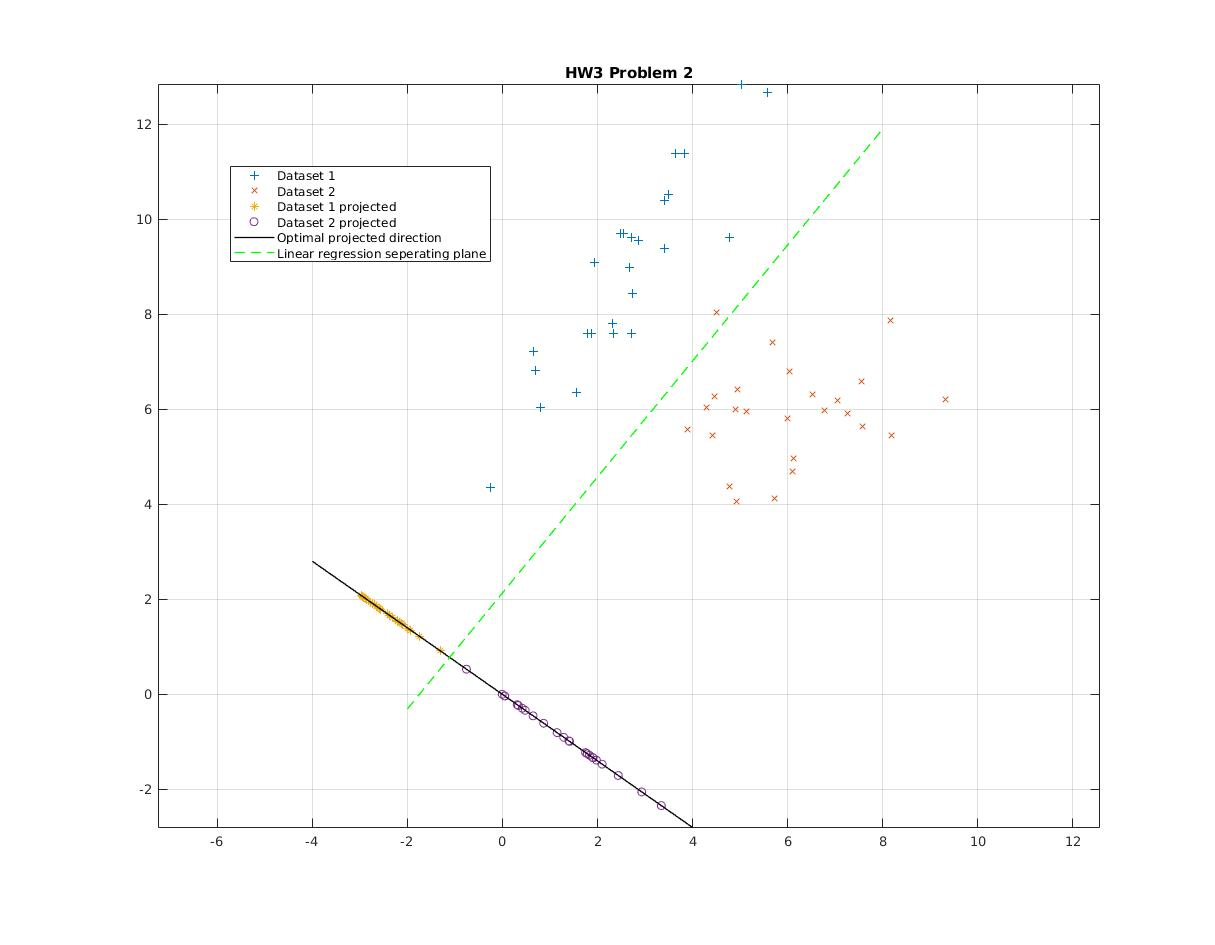
\includegraphics[width=1\textwidth]{images/untitled.jpg}
 \end{center}
\end{figure}

\textit{Comments:}
Linear regression classifier has slightly worse performance than Fisher discriminator in this case (wrongly classify one point). 
% --------------------------------------------------------------
%     You don't have to mess with anything below this line.
% --------------------------------------------------------------
 
\end{document}